\documentclass[11pt,a4paper,openany,leqno]{article}

\textwidth=160mm \textheight=260mm \hoffset=-18mm \voffset=-30mm
\setcounter{page}{1}
			\usepackage[magyar]{babel}
			\usepackage[utf8]{inputenc}
			\usepackage[T1]{fontenc}
			\usepackage{indentfirst}
			\usepackage{amsmath,esint}
			\usepackage{amssymb}
%			\usepackage{eufrak}
			\usepackage{psfrag}
			\usepackage{tabularx}
			\usepackage{graphicx}
			\usepackage{wrapfig}	
			\usepackage{hyperref}
			\usepackage{multicol}	
									
			\frenchspacing
			\allowhyphens

\tolerance=2000
\hbadness=2000
\vbadness=10000
\overfullrule=0pt




\begin{document}
\section{Ampere-törvény, Lorentz-erő}
\subsection{2. ZH 2018 2.feladat}


Egymással párhuzamos homogén $E$ elektromos és $B$ mágneses térben mozog egy m tömegű,
Q töltésű részecske. Indítsuk el a részecskét $v$ nagyságú és a terekre merőleges irányú sebességgel. Milyen messze lesz a részecske az indulási pontjától $\frac{m\cdot \pi}{Q\cdot B}$ idő múlva?\\ \indent
{\it Segítség: Ne csinálj Lorentz-transzformációt!}

\begin{figure}[h!]
\centering
  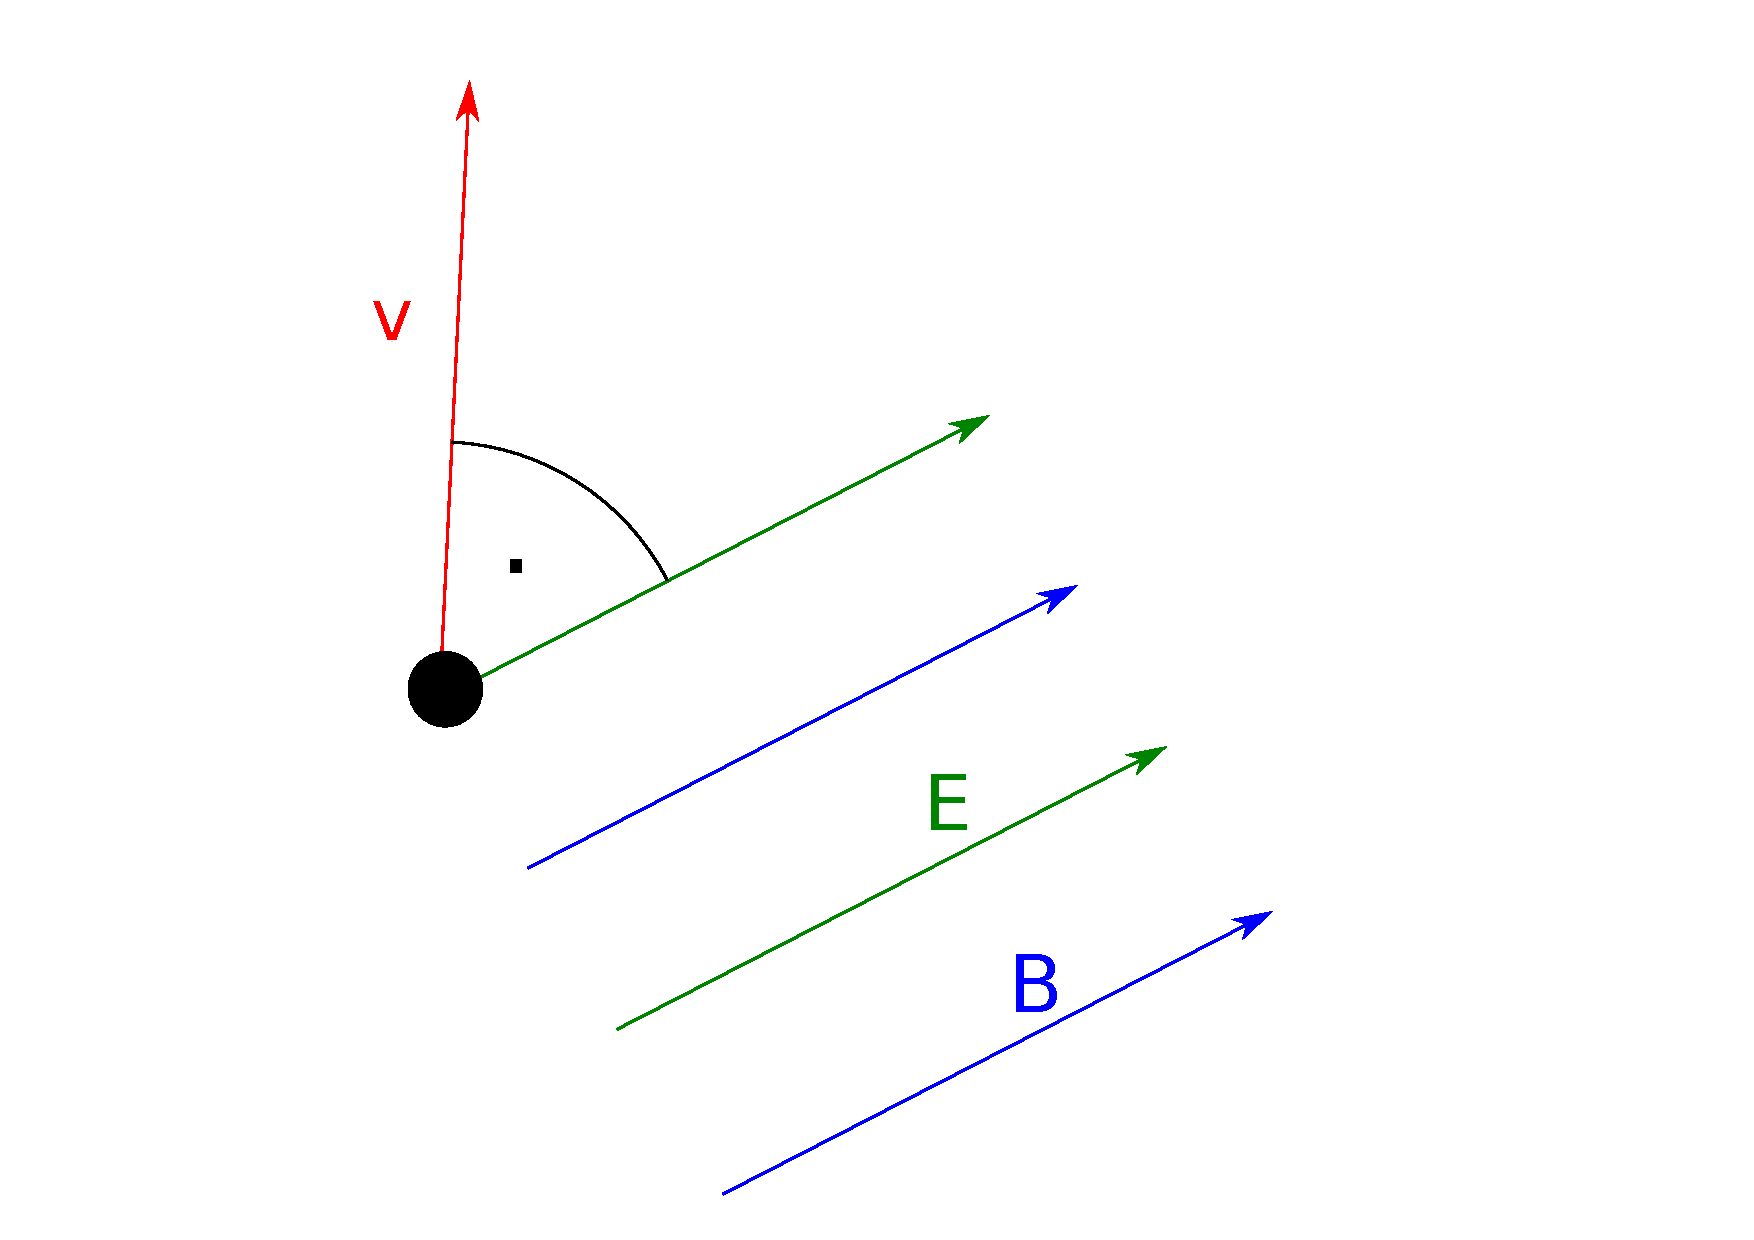
\includegraphics[width=120mm,scale=0.5]{abra.pdf}
  \caption{Az elektromos és a mágneses térre merőleges sebességű}
  \label{}
\end{figure} 


\begin{flushright} {Feladatot kidolgozta: {\it Z2R8XS}} \end{flushright}

\vspace{0.5cm}

\textbf{Megoldás}\\
\indent
Legyen koordinátarenszer origója a töltés helyzete a $t=0$ pillanatban. A $z$ tengely legyen párhuzamos az elektromos, illetve a mágneses térerősség vektorával, az $x$ tengely pedig a $\vec{v}_0$ sebesség vektorral.\\ \indent
A Lorentz-erő
$$ \vec{F} = Q(\vec{E} + \vec{v} \times \vec{B}) $$
\indent{}
minden időpillanatban. Newton törvényeiből
$$ m \cdot\vec{r''}(t) = Q(\vec{E} + \vec{r'}(t) \times \vec{B}) $$
\indent
Ez egy differenciál egyenlet rendszer $\vec{r}$ komponenseire. Ebben a koordinátarendszerben $\vec{E}$ és $\vec{B}$ konstans vektorok.\\ \indent
$$ \begin{pmatrix} x'' \\ y'' \\ z''  \end{pmatrix} = \frac{Q}{m} \cdot (\begin{pmatrix} 0 \\ 0 \\ E  \end{pmatrix} + \begin{pmatrix} x' \\ y' \\ z'  \end{pmatrix} \times \begin{pmatrix} 0 \\ 0 \\ B  \end{pmatrix}) $$

$$ \begin{pmatrix} x'' \\ y'' \\ z''  \end{pmatrix} = \frac{Q}{m} \cdot (\begin{pmatrix} 0 \\ 0 \\ E  \end{pmatrix} + \begin{pmatrix} B\cdot y' \\- B\cdot x' \\ 0  \end{pmatrix})  $$
\indent A differenciál egyenlet rendszer így
$$ x'' = \frac{Q}{m}\cdot B \cdot  y' $$
$$ y'' = -\frac{Q}{m}\cdot B \cdot  x' $$
$$ z'' = \frac{Q}{m}\cdot E $$ \indent
Megsejthető, hogy $x(t)$ és $y(t)$ valamiféle $sin$-okból és $cos$-okból állhat. Ha csak mágneses tér lenne, akkor egyszerű síkmozgást (körmozgást) szeretne végezni a test. Ha csak elektromos tér lenne, a térerősség irányába gyorsulna a test. Ebben az esetben mindkét mozgás típus jelen van - és ezek összeadhatók. Az összeadást jogosítja az, hogy az elektromos tér számára $\vec{v}$-nek csak a térrel párhuzamos komponense fontos, a mágneses térnek pedig csak a merőleges komponens fontos (a kereszt szorzat miatt). Így az elektromos tér csak a $z$ komponensbe szól bele, a mágneses pedig a másik kettőbe.\\ \indent
Rendelkezésre álló kezdőfeltételek:\\ \indent
A töltés $t=0$ pillanatban az origóban van.\\
$$ x(0) = 0 $$
$$ y(0) = 0 $$
$$ z(0) = 0 $$
\indent
A töltés sebessége $t=0$ pillanatban az $x$ tengely irányába mutat.\\
$$ x'(0) = v_0 $$
$$ y'(0) = 0 $$
$$ z'(0) = 0 $$
\indent
Hat kezdőfeltétel három másodrendű differenciál egyenlethez elég.\\ \indent
\medskip
Az $x$ függvény nulla, ha $t=0$, valamint $x'$ nem nulla. Ez úgy viselkedik ebben a pontban, mint a $j\cdot sin(k\cdot t)$ függvény.\\ \indent
Az $y$ függvény nulla, ha $t=0$, valamint $y'$ is nulla. Ez $(-j)\cdot cos(k\cdot t) + konstans$-ként viselkedik.\\ \indent
Ennek az a fizikai értelme, hogy a koordinátarendszer origója rögzítve van a kezdeti helyzethez, de nem az origó körül fog forogni a töltés, hanem egy $\vec{B}$-vel párhuzamos tengely körül, amely $R$ távolságra van az origótól.\\ \indent
A Lorentz-erő szolgáltatja a centirpetális erőt a körmozgáshoz. A centripetális gyorsulás nagysága\\ 
$$ a_{cp} = \frac{v_{(x,y)}^2}{R} $$\indent
Ha a töltés mozgása $(x,y)$ síkra levetítve körmozgás, akkor van egy konstans $\omega$ szögsebessége (ez lesz a $k$ együttható), és $\vec{v}$-nek nem változik a nagysága, ha levetítjük az $(x,y)$ síkra. Így a képletbe beírható a kezdősebesség. Mivel pozitív $x$ irányú a kezdősebesség, algebrailag a kör egyenlete $x^2 + (y-R)^2 = R^2$. Az $y(t)$ függvénynek tehát tartalmaznia kell egy "$+R$" tagot - ez a konstans lesz hozzáadva a koszinuszhoz.\\ 
$$ x=R\cdot sin(\omega \cdot t) $$
$$ y=-R\cdot cos(\omega \cdot t) + R $$\indent
Ez a két függvény megfelel a kezdőfeltételeknek, ha $R \cdot \omega = v_0$, és a kör egyenletét is kielégítik.\\ \indent
Hiányzik még $R$ és $\omega$ értéke.\\
$$ x'' = \frac{Q}{m}\cdot B \cdot  y' $$
$$ -\omega^2 \cdot R\cdot sin(\omega \cdot t) = \frac{Q}{m}\cdot B \cdot (-R \cdot \omega \cdot sin(\omega \cdot t))  $$
$$ \omega = \frac{Q}{m}\cdot B $$
$$ R = \frac{m\cdot v_0}{Q\cdot B} $$ \indent
Ezeket az értékeket visszakapjuk az $y(t)$ második deriváltjára vonatkozó egyenletből is.\\ \indent
Ellenőrizzük le, hogy a centripetális gyorsulás esetén sem futunk ellentmondásba.\\ 
$$ a_{cp} = \sqrt{(x'')^2 + (y'')^2} $$
$$ \frac{v_0^2}{R} = \sqrt{\omega^4 \cdot R^2 \cdot sin^2(\omega \cdot t) + \omega^4 \cdot R^2\cdot cos^2(\omega \cdot t)} $$
$$ v_0^2 = R^2 \cdot \omega^2 $$ \indent
Az alábbiak lesznek az $x(t)$ és az $y(t)$ függvények.
$$ x(t) = \frac{m\cdot v_0}{Q\cdot B}\cdot sin(\frac{Q}{m}\cdot B \cdot t) $$
$$ y(t) = \frac{- m\cdot v_0}{Q\cdot B} \cdot cos(\frac{Q}{m}\cdot B \cdot t) + \frac{m\cdot v_0}{Q\cdot B} $$ \indent
A $z(t)$ függvény maradt utoljára. Második deriváltja konstans, első deriváltja $t=0$ helyen $0$, és $z(0)=0$, így a függvény $c\cdot t^2$ alakú lesz. \\
$$ z(t) = \frac{Q}{m}\cdot E \cdot t^2 $$  \indent
Az $r(t)$ függvényre van még szükség. Ez az $\vec{r}(t)$ vektor hossza.\\
$$ r(t) = \sqrt{x^2(t) + y^2(t) + z^2(t)} $$
$$ r(t) = \sqrt{\frac{m^2\cdot v_0^2}{Q^2\cdot B^2}\cdot sin^2(\frac{Q}{m}\cdot B \cdot t) + (\frac{- m\cdot v_0}{Q\cdot B} \cdot cos(\frac{Q}{m}\cdot B \cdot t) + \frac{m\cdot v_0}{Q\cdot B})^2 + \frac{Q^2}{m^2}\cdot E^2 \cdot t^4} $$ \indent
A feladat az $r(\frac{m \cdot \pi}{Q \cdot B})$ értéket kéri.\\
$$ r(\frac{m \cdot \pi}{Q \cdot B}) = \sqrt{\frac{m^2\cdot v_0^2}{Q^2\cdot B^2}\cdot sin^2(\frac{Q}{m}\cdot B \cdot \frac{m \cdot \pi}{Q \cdot B}) + (\frac{- m\cdot v_0}{Q\cdot B} \cdot cos(\frac{Q}{m}\cdot B \cdot \frac{m \cdot \pi}{Q \cdot B}) + \frac{m\cdot v_0}{Q\cdot B})^2 + \frac{Q^2}{m^2}\cdot E^2 \cdot (\frac{m \cdot \pi}{Q \cdot B})^4} $$

$$ r(\frac{m \cdot \pi}{Q \cdot B}) = \sqrt{\frac{m^2\cdot v_0^2}{Q^2\cdot B^2}\cdot sin^2(\pi) + (\frac{- m\cdot v_0}{Q\cdot B} \cdot cos(\pi) + \frac{m\cdot v_0}{Q\cdot B})^2 + \frac{Q^2}{m^2}\cdot E^2 \cdot (\frac{m \cdot \pi}{Q \cdot B})^4} $$

$$ r(\frac{m \cdot \pi}{Q \cdot B}) = \sqrt{\frac{Q^2}{m^2}\cdot E^2 \cdot \frac{m^4 \cdot \pi^4}{Q^4 \cdot B^4}} $$
$$ r(\frac{m \cdot \pi}{Q \cdot B}) = \sqrt{\frac{E^2 \cdot m^2 \cdot \pi^4}{Q^2 \cdot B^4}} $$
$$ r(\frac{m \cdot \pi}{Q \cdot B}) = \frac{E \cdot m \cdot \pi^2}{Q \cdot B^2} $$
 Tehát a töltés a $t=\frac{m \cdot \pi}{Q \cdot B}$ idő múlva $\frac{E \cdot m \cdot \pi^2}{Q \cdot B^2}$ távolságra lesz az iniciális helyzetétől.



\end{document}